\documentclass[aspectratio=169]{beamer}
\mode<presentation>
%\usetheme{Warsaw}
%\usetheme{Goettingen}
\usetheme{Hannover}
%\useoutertheme{default}

%\useoutertheme{infolines}
\useoutertheme{sidebar}
\usecolortheme{dolphin}


\setbeamersize{sidebar width left=0pt} % to remove the sidebar
\beamertemplatenavigationsymbolsempty % To remove the navigation symbols on the bottom right.
\setbeamersize{text margin left=10mm,text margin right=10mm} % Specify margins

\usepackage{amsmath}
\usepackage{amssymb}
\usepackage{listings}
\usepackage{enumerate}
\usepackage{hyperref}
\hypersetup{
    colorlinks=true,
    linkcolor=blue,
    filecolor=magenta,      
    urlcolor=cyan,
}
 
\urlstyle{same}

%some bold math symbosl
\newcommand{\Cov}{\mathrm{Cov}}
\newcommand{\Var}{\mathrm{Var}}
\newcommand{\brho}{\boldsymbol{\rho}}
\newcommand{\bSigma}{\boldsymbol{\Sigma}}
\newcommand{\btheta}{\boldsymbol{\theta}}
\newcommand{\bbeta}{\boldsymbol{\beta}}
\newcommand{\bmu}{\boldsymbol{\mu}}
\newcommand{\bW}{\mathbf{W}}
\newcommand{\one}{\mathbf{1}}
\newcommand{\bH}{\mathbf{H}}
\newcommand{\by}{\mathbf{y}}
\newcommand{\bolde}{\mathbf{e}}
\newcommand{\bx}{\mathbf{x}}

\newcommand{\cpp}[1]{\texttt{#1}}

%--------------------------------------------------
\providecommand{\abs}[1]{\lvert#1\rvert}
\providecommand{\norm}[1]{\lVert#1\rVert}
\providecommand{\Blue}[1]{\textcolor{blue}{#1}}
\providecommand{\Red}[1]{\textcolor{red}{#1}}
\newcommand{\celsius}{\ensuremath{^\circ}C}
\newcommand\thfore{\mathord{\therefore}\,}
%------------------------------------------------------------------

\title{Lecture 8. Planar Graphs}
%\author{\includegraphics[width=.5\textwidth,height=.5\textheight]{lecture8-fig1.png}}

\date{ }
%------------------------------------------------------------------


\begin{document}

\frame[plain]{\titlepage}

\begin{frame}[plain]{}

Consider the problem of joining three houses to each of three separate utilities.
 Is it possible to join these houses and utilities such that none of the connections cross?
 
 \begin{center}
  \includegraphics[width=.5\textwidth,height=.5\textheight]{./img/lecture8-fig1.png}
 \end{center}
 
 \pause
 
 \medskip
 
 {\bf Definition.} A graph is called \Blue{planar} if it can be drawn \Red{on the plane} 
    in such a way that no edges cross each other. 
\end{frame}

\begin{frame}[plain]{}


 \begin{center}
  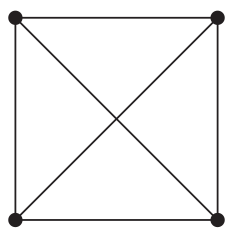
\includegraphics[height=3cm]{./img/lecture8-fig2.png}\pause \ \ \ \ \ \ \ \ 
  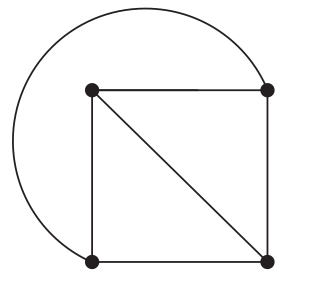
\includegraphics[height=3cm]{./img/lecture8-fig3.png}\pause 
 \end{center}
 \medskip
 
 \begin{center}
  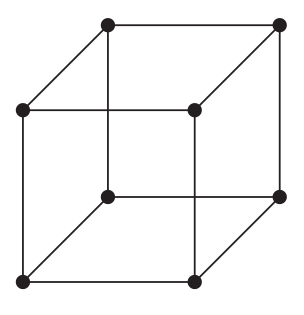
\includegraphics[height=3cm]{./img/lecture8-fig4.png}\pause \ \ \ \ \ \ \ \ 
  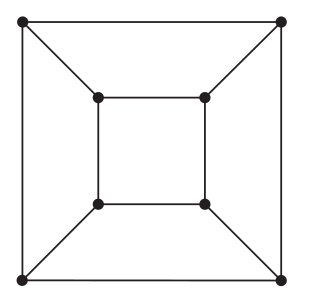
\includegraphics[height=3cm]{./img/lecture8-fig5.png}
 \end{center}
 
\end{frame}

\begin{frame}[plain]{}

{\bf Example 8.1.} Show that a complete bipartite graph $K_{3,3}$ is not a planar graph.
  \begin{center}
  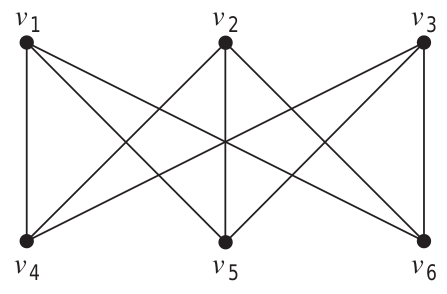
\includegraphics[height=3cm]{./img/lecture8-fig6.png}\pause \ \ \ \ \ \ \ \ 
  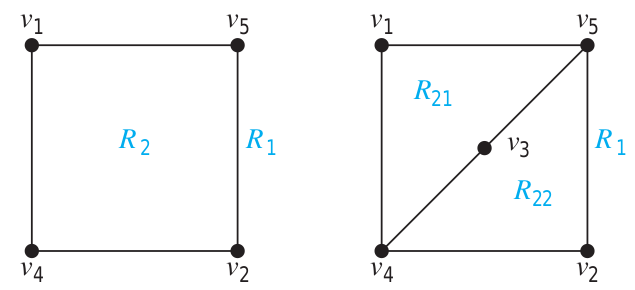
\includegraphics[height=3cm]{./img/lecture8-fig7.png} \ \ \\
   \ \ \ \ \ \ \ \ \ \ \ \ \ \ \ \ \ \ \ \ \ \ \ \ \
   \ \ \ \ \    Where to put $v_6$?
 \end{center}
 
 \begin{center}
   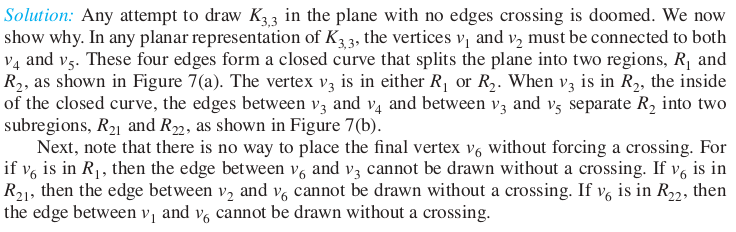
\includegraphics[height=3.5cm]{./img/lecture8-fig10.png}
 \end{center}
 
\end{frame}


\begin{frame}[plain]{}

{\bf Practice 8.2.} Determine if the given graph is planner by
 drawing the graph without any crossings.
 
 \begin{center}
   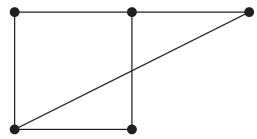
\includegraphics[height=2cm]{./img/lecture8-fig13a.png}
   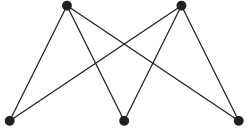
\includegraphics[height=2cm]{./img/lecture8-fig13b.png}
   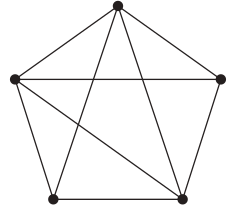
\includegraphics[height=2cm]{./img/lecture8-fig13c.png}
 \end{center}
 \vspace{1.3in}
 
\end{frame}

\begin{frame}[plain]{Euler Characteristic of A Planar Graph}

A planar representation of a graph splits the plane into regions,
 including an unbounded region.
For instance, the planar representation of the graph shown in Figure 
 splits the plane into six
regions.

\begin{center}
   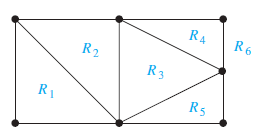
\includegraphics[height=2.3cm]{./img/lecture8-fig9.png}
 \end{center}
 \pause
 

{\bf Definition.} Let $G$ be a planar graph with $e$ edges and 
$v$ vertices. Let $r$ be the number of regions in a planar representation of $G$.
The quantity \Blue{$v-e+r$} is called the \Blue{Euler characteristic} of the graph $G$.
\smallskip

{\bf Example 8.3.} What is the Euler characteristic of the graph in the above picture?

 \end{frame}

\begin{frame}[plain]{ }

{\bf Definition.} Let $G$ be a planar graph with $e$ edges and 
$v$ vertices. Let $r$ be the number of regions in a planar representation of $G$.
The quantity \Blue{$v-e+r$} is called the \Blue{Euler characteristic} of the graph $G$.
\smallskip

{\bf Example 8.4.} Find the Euler characteristic of the graphs below, if possible.
 
 \begin{center}
   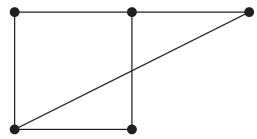
\includegraphics[height=2cm]{./img/lecture8-fig13a.png}
   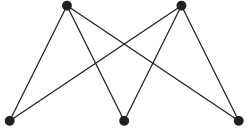
\includegraphics[height=2cm]{./img/lecture8-fig13b.png}
   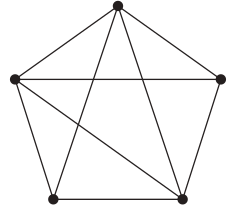
\includegraphics[height=2cm]{./img/lecture8-fig13c.png}
 \end{center}

\pause

{\bf Question.} Any observation from Examples 8.3 and 8.4?
\pause

\medskip

{\bf Theorem 8.5} (Euler's Formula). For any connected planar
graph,  \Blue{$v-e+r = 2$.}
\medskip
\pause 

{\bf Example 8.6.} Suppose that a connected planar simple graph has 
20 vertices, each of degree 3. Into how many
regions does a representation of this planar graph split the plane?

 \end{frame}

\begin{frame}[plain]{}

 {\bf Theorem 8.7}  If a connected planar simple graph has  $e$ edges 
 and $v$ vertices with $v\geq 3$, then $e\leq 3v-6$.
 \medskip
 
 {\bf Theorem 8.8.} If a connected planar simple graph has  $e$ edges, 
 $v$ vertices with $v\geq 3$ and no circuits of length three, then $e\leq 2v-4$.
 \medskip
 
 {\bf Example 8.9.}
 $K_{3,3}$ satisfies Theorem 8.7 but not Theorem 8.8. Thus, $K_{3,3}$ is nonplanar.
 \medskip
 
 {\bf Practice 8.10.}  Determine whether the given graph is planar.
 If so, draw it so that no edges cross.
\begin{center}
  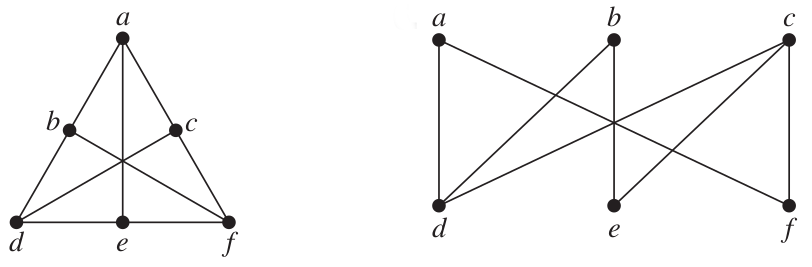
\includegraphics[height=2.5cm]{./img/lecture8-fig11.png}
 \end{center}
 
\end{frame}

\begin{frame}[plain]{}
 
 {\bf Activity 8.11}. Show that a complete graph $K_{5}$ is not a planar graph using 
a similar argument to that given in Example 8.1.
 \begin{center}
   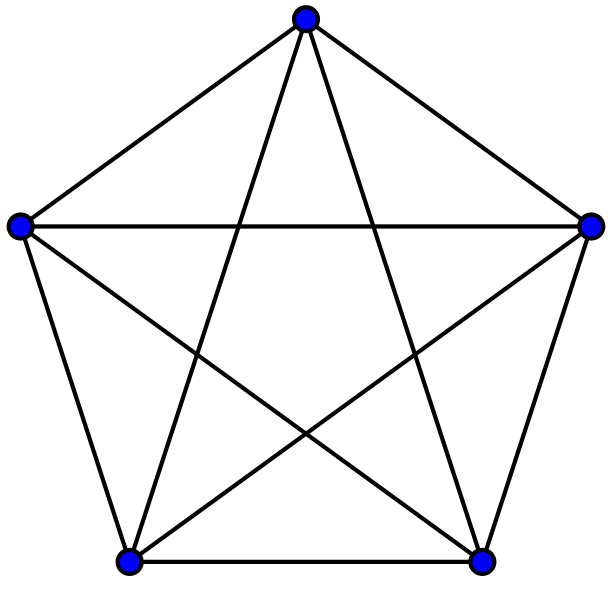
\includegraphics[height=2.5cm]{./img/lecture8-fig8.png}
 \end{center}
\vspace{1in}

 
\end{frame}



\end{document}
%%%%%%%%%%%%%%%%

\begin{frame}[plain]{}

{\bf Exercise 8.11.}  Determine whether the given graph is planar.
 If so, draw it so that no edges cross.
\begin{center}
  \includegraphics[height=2.5cm]{lecture7-fig12.png}
 \end{center}
\vspace{1in}

\end{frame}





%%%%%%%%%%%%%%%%%%%%%
 